\chapter{Experiments and Evaluations}
\label{ch:experiments}

This chapter presents details of the experiments and evaluations for the proposed test scripts in the previous chapter.
First, we describe the environment setup for testing process.
Subsequently, we present all the experiments along with evaluation and assessment for each of them.

\section{Experimental environment}

\subsection{Hardware configurations}
All test suites are conducted with the hardware configurations as shown in table \ref{tab:hw}. We use 2 phones running 2 different \acrshort{os} versions with different screen size and resolution for testing the portability of the system.

\begin{table}[H]
	\centering
	\caption{Hardware configuration for testing process}	
	\label{tab:hw}
	\begin{tabularx}{0.65\textwidth}{ll}
		\toprule
		Phone 1 & ASUS Zenfone 5 \\
			  & Resolution 720 x 1280 pixels \\
			  & Screen 5'' 6.22 cm x 11.06 cm \\
			  & Android 5.0.1\\
		\midrule 
		Phone 2 & Sony XPeria L \\
			  & Resolution 480 x 850 pixels \\
			  & Screen 4.3'' 5.40 cm x 9.60 cm \\
			  & Android 4.2.2\\
		\midrule 
		Robot & Self-construct Delta Robot \\
			  & \begin{minipage}{0.7\linewidth}
			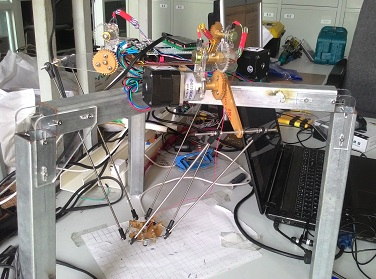
\includegraphics[width=0.8\linewidth]{Chapters/Fig/delta_robot.jpg}
		\end{minipage} \\
		\midrule 
		Computer & Windows computer \\
				 & Having 2 USB ports for connecting the phone and the robot. \\
		\bottomrule
	\end{tabularx}
\end{table}

\subsection{Supporting software}
The application can not operate lonely. It requires some supporting software on the computer and applications to be tested installed on target phones.

	\begin{itemize}
		\item[--] \textbf{Android platform tool}: command line tools for communicate with Android device.
		\item[--] \textbf{Droid@Screen}: application letting us capture Android screen to PC.
		\item[--] \textbf{Simple Click Test} \footnote{Source code available at: \url{https://github.com/alfrededison/simple-click-test}}: self-created tested application for Experiment 1.
		\item[--] \textbf{Clock ICS} \footnote{Download available at Google Play Store: \url{https://play.google.com/store/apps/details?id=com.moblynx.clockics}}: tested application for Experiment 2.
	\end{itemize}

\subsection{Experimental procedure}
First, set the phone to the calibrated position of the robot's pointer.

	\begin{figure}[H]
		\centering
		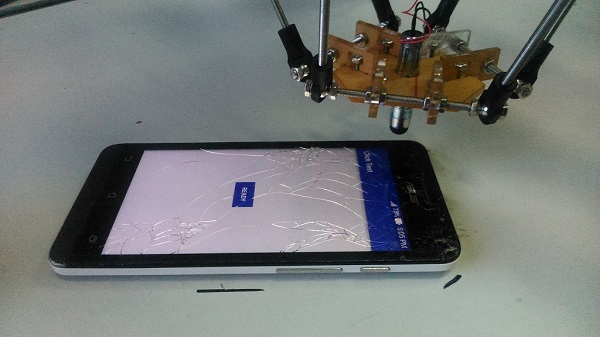
\includegraphics[scale=0.5]{Chapters/Fig/phone_setup.jpg}
		\caption{Setup phone position}
		\label{fig:phone_setup}
	\end{figure}

Then open Droid@Screen application to capture phone screen. See Appendix \ref{ch:img_capture} for capturing process's detail.

	\begin{figure}[H]
		\centering
		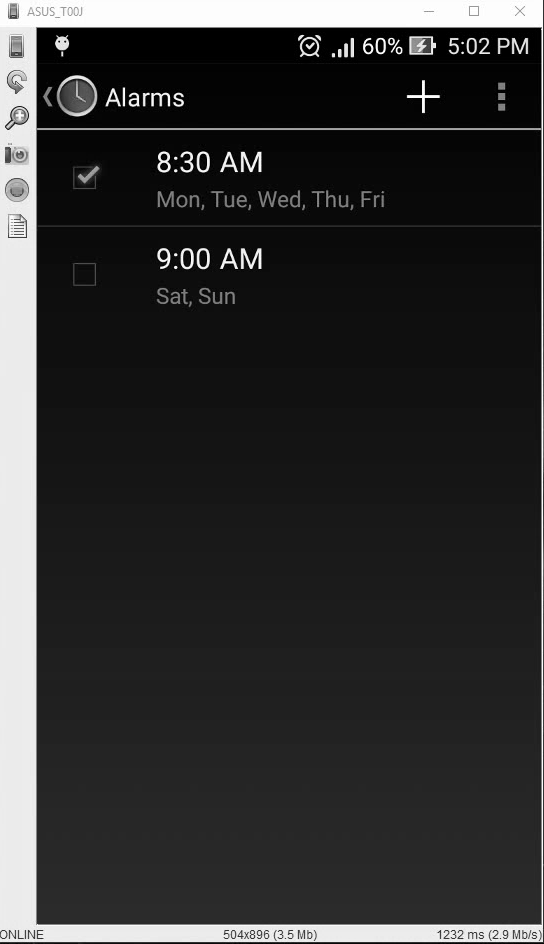
\includegraphics[scale=0.5]{Chapters/Fig/droidscreen.png}
		\caption{Capture phone screen}
		\label{fig:droidscreen}
	\end{figure}

Finally, open the program and set up the parameters

	\begin{figure}[H]
		\centering
		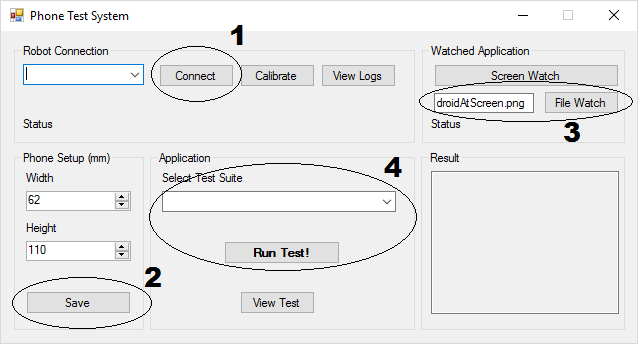
\includegraphics[scale=0.5]{Chapters/Fig/prog_setup.png}
		\caption{Parameter setup}
		\label{fig:prog_setup}
	\end{figure}

	\begin{itemize}
		\item[--] Connect to the robot by choosing COM port and press Connect.
		\item[--] Configure phone size
		\item[--] Choose screen watching method
		\item[--] Select test suite and run the test
	\end{itemize}

\section{Experiments and Results}
This section gives the details of all experiments that we have conducted to verify and evaluate the accuracy of Delta robot as well as the whole Testing System proposed in the previous chapter.

\subsection{Experiment 1: Test robot accuracy}
\subsubsection{Experimental purpose}
By letting the Delta robot move around the phone screen, we can test the working accuracy of the robot under certain repeated actions.

\subsubsection{Experimental setup}
	\begin{itemize}
		\item[--]Open Click test application on the phone. Let the application be at initial page.
		\item[--]Follow the experimental procedure mentioned in previous section.
	\end{itemize}

\subsubsection{Experimental results}
Begin test screen, the robot need to click on READY button.
	\begin{figure}[H]
		\centering
		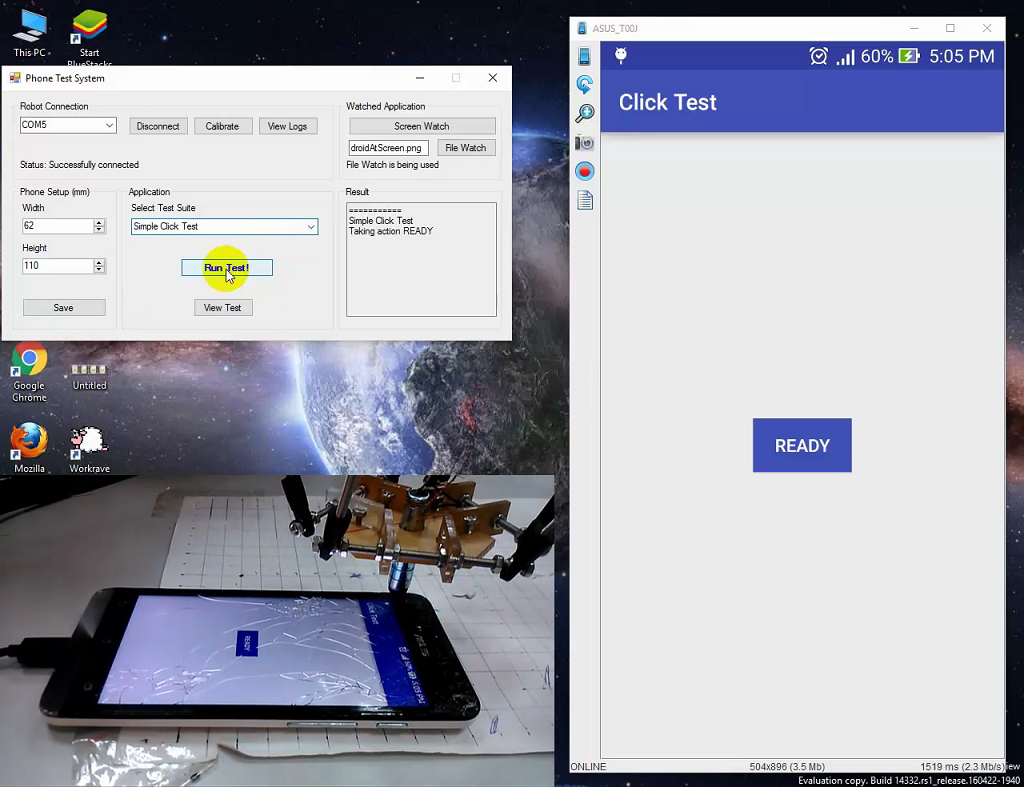
\includegraphics[scale=0.5]{Chapters/Fig/click_start.png}
		\caption{Begin click test screen}
		\label{fig:click_start}
	\end{figure}

After clicking on READY, SUCCESS button appears. The robot is commanded to click on it.

	\begin{figure}[H]
		\centering
		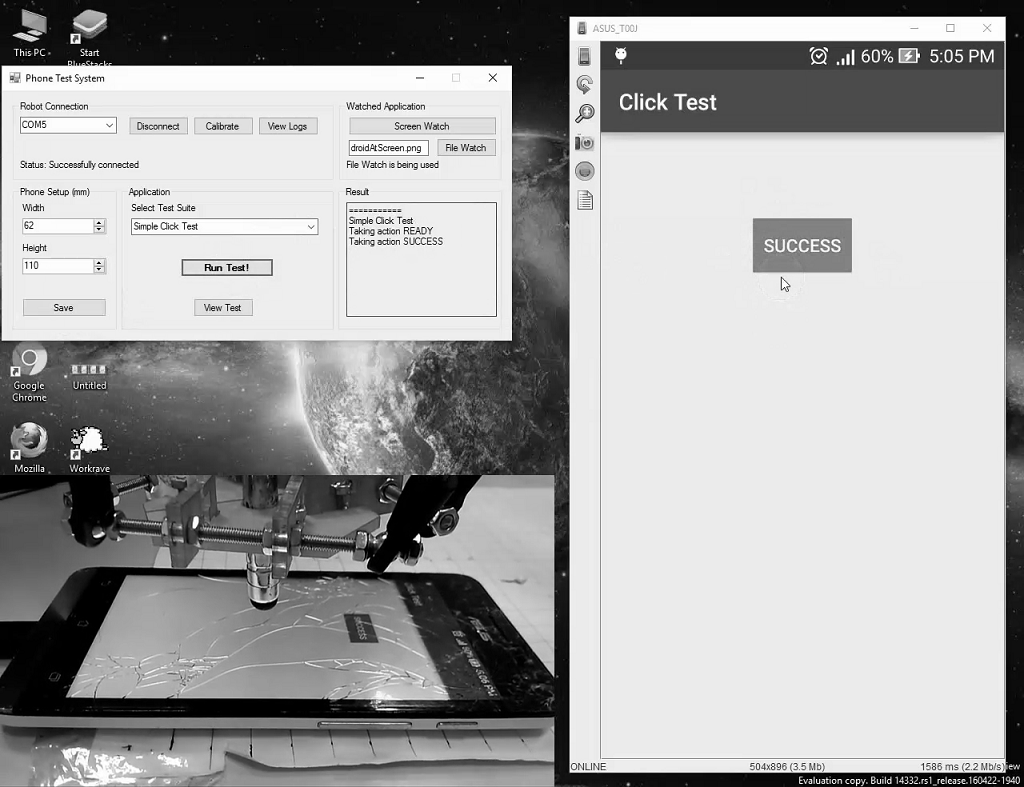
\includegraphics[scale=0.5]{Chapters/Fig/click_mid.png}
		\caption{After clicking READY screen}
		\label{fig:click_mid}
	\end{figure}

Final result when READY is clicked. The test is passed.
	\begin{figure}[H]
		\centering
		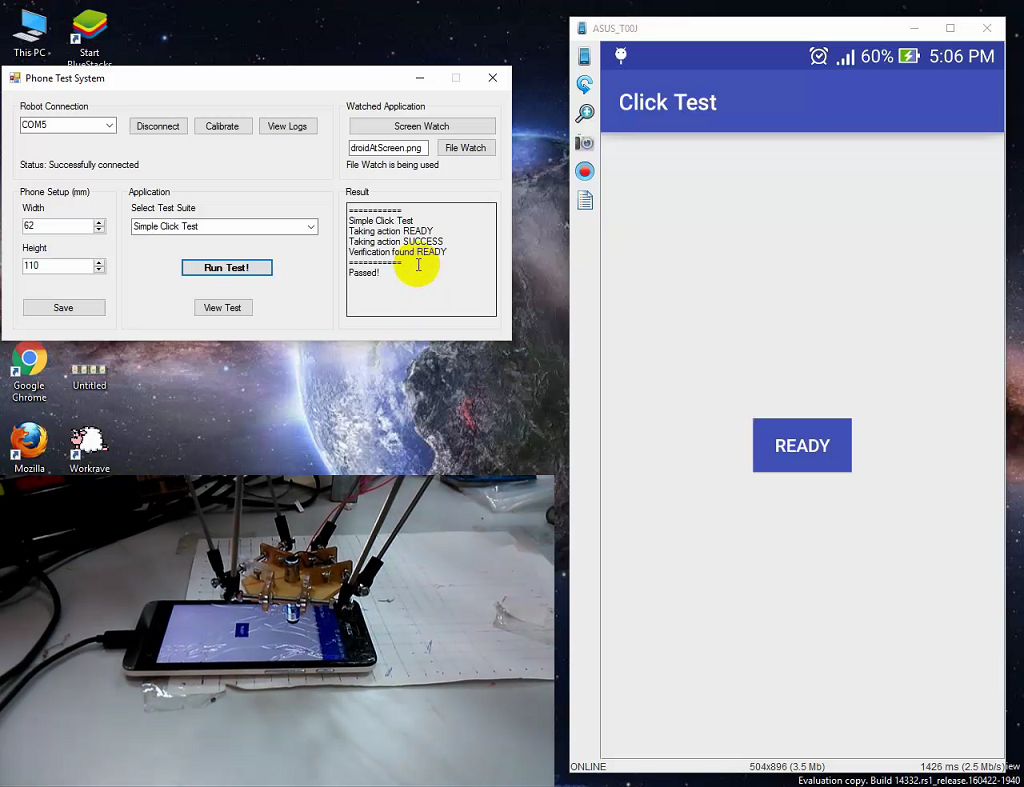
\includegraphics[scale=0.5]{Chapters/Fig/click_final.png}
		\caption{Final click test screen}
		\label{fig:click_final}
	\end{figure}

\subsection{Experiment 2: Set alarm}
\subsubsection{Experimental purpose}

\subsubsection{Experimental setup}
Open Clock ICS application. Then open set alarm item.

\subsubsection{Experimental results}
Begin test
	\begin{figure}[H]
		\centering
		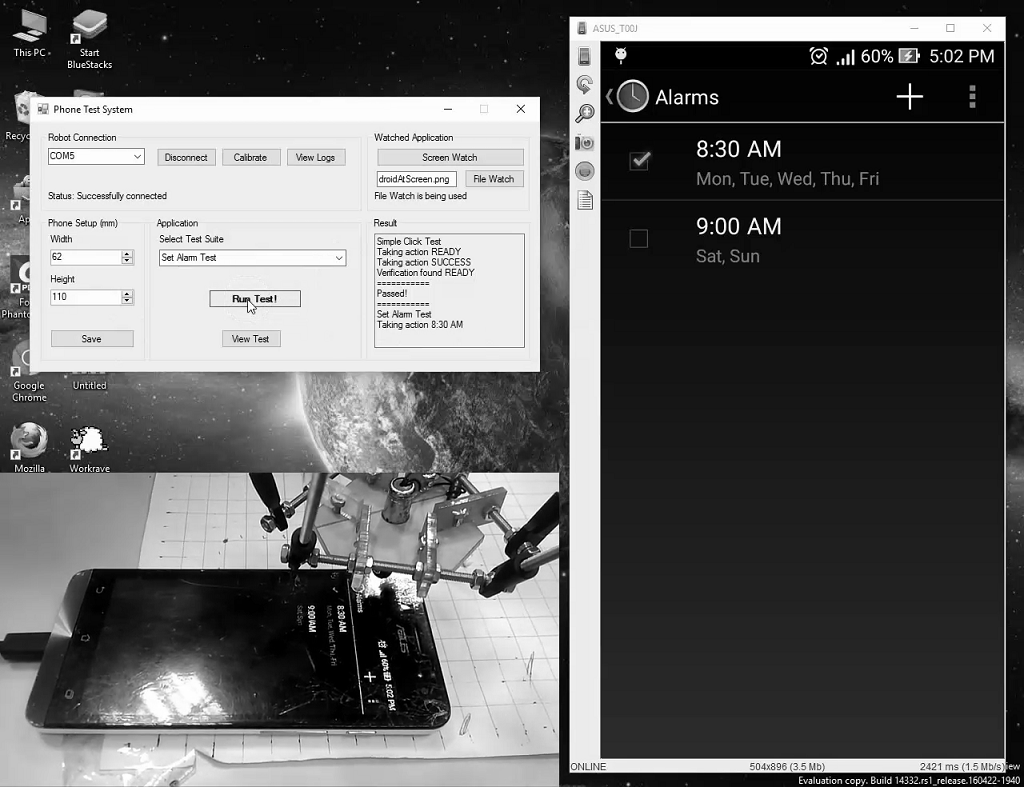
\includegraphics[scale=0.5]{Chapters/Fig/alarm_start.png}
		\caption{begin alarm test}
		\label{fig:alarm_start}
	\end{figure}

Final result
	\begin{figure}[H]
		\centering
		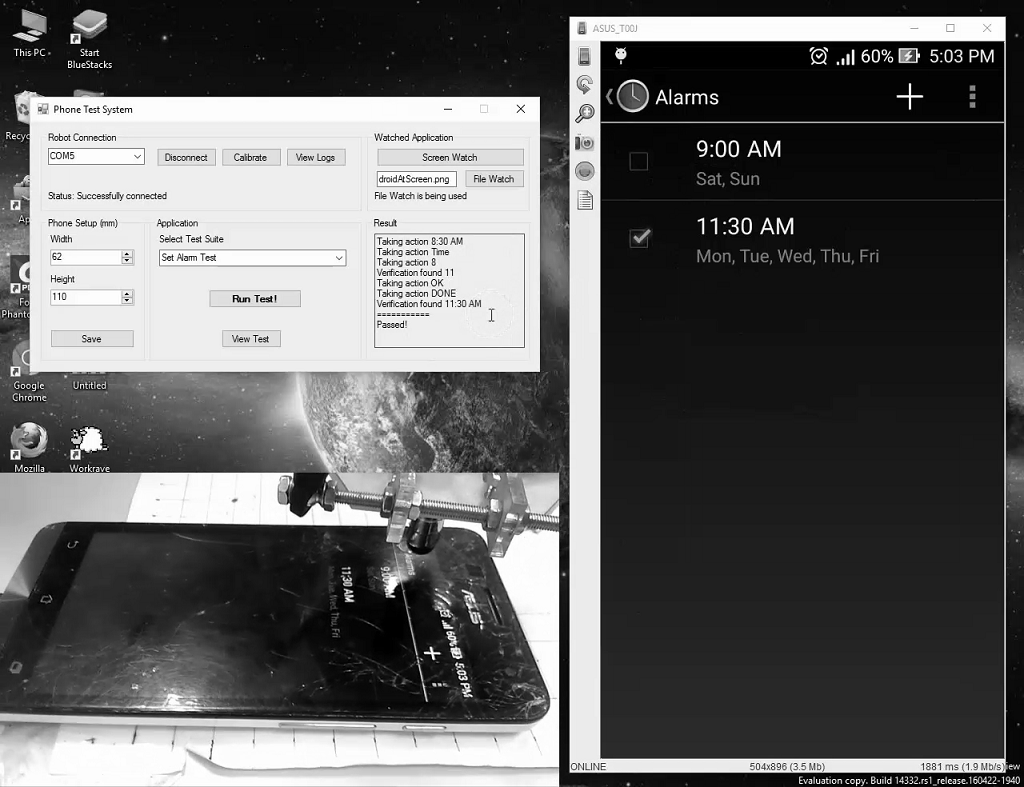
\includegraphics[scale=0.5]{Chapters/Fig/alarm_final.png}
		\caption{final alarm test}
		\label{fig:alarm_final}
	\end{figure}

\section{Analysis and evaluation}
\subsection{Results analysis}
\begin{table}[H]
	\centering
	\caption{Test results statistic}	
	\label{tab:result_stat}
	\begin{tabularx}{0.65\textwidth}{l|rrr}
		\hline
		Test case & Successful & Failed & Number of tests \\
		\hline
		Simple Click & 10 & 0 & 10 \\
		Set Alarm & 5 & 5 & 10 \\
		\hline
		Total & 15 & 15 & 20 \\
		\hline
		\textbf{Rate} & \textbf{0.50} & \textbf{0.50} & \textbf{1.00} \\
		\hline
	\end{tabularx}
\end{table}

\subsection{Conclusion:}
Conclusion here
